% !Mode:: "TeX:UTF-8"
% !TEX program  = xelatex
\section{Related Work}
This chapter is based on the requirements of realizing image segmentation on the mobile terminal, I studied the classical FCN \cite{long2015fully} semantic segmentation algorithm and the FPN-based FaPN \cite{huang2021fapn} algorithm, analyze the problems running on the mobile terminal and choose to improve the FaPN model. After comparing MobileNet V3 and Paddle Lite \cite{paddlelite}, the Paddle Lite network was selected as the model for mobile semantic segmentation using the computing power of the mobile phone AI chip. 

% \subsection{Fully Convolutional Network}
% The FCN network structure \cite{long2015fully} was proposed by Jonathan Long et al. in 2014. Before this, the CNN network usually connects several fully connected layers after the convolutional layer and maps the feature map generated by the convolutional layer into a fixed-length feature vector. Each value of this output vector represents the probability that the input image belongs to a given class. The semantic segmentation network of the FCN network is constructed based on the convolutional neural network. The calculation in the network is the same as that in the convolution upgrade network, and there are convolutional layers, pooling layers, and activation function layers.

% Unlike classical CNNs that use fully connected layers after convolutional layers to obtain fixed-length feature vectors for classification, FCNs can accept input images of any size. FCN uses the deconvolution layer to upsample the feature map of the last convolution layer to restore it to the same size as the input image so that a prediction can be generated for each pixel while retaining the original input image. Spatial information, and finally perform pixel-wise classification on the upsampled feature map.

% The structure of the traditional CNN network is to add 4096, 4096, and 1000 channels of fully connected layers after the convolutional layer for the final predicted output. Among them, AlexNet and VGG16 are represented, which are mainly used for image classification tasks.


% \begin{figure}[htbp]
%     \centering
%     \begin{subfigure}[t]{1\linewidth}
%         \centering
%         \includegraphics[width=1\textwidth]{figures/CNN.png}
%         \caption{Typical CNN structure: usually, the CNN network will be connected to several fully connected layers after the convolutional layer, and the feature map generated by the convolutional layer will be mapped into a fixed-length feature vector. For all image-level classification and regression tasks, they expect a numerical description of the entire input image at the end. For example, AlexNet [18] outputs a 1000-dimensional vector indicating that the input image belongs to probability of which class.}\label{CNN}
%     \end{subfigure}
%     \begin{subfigure}[t]{1\linewidth}
%         \centering
%         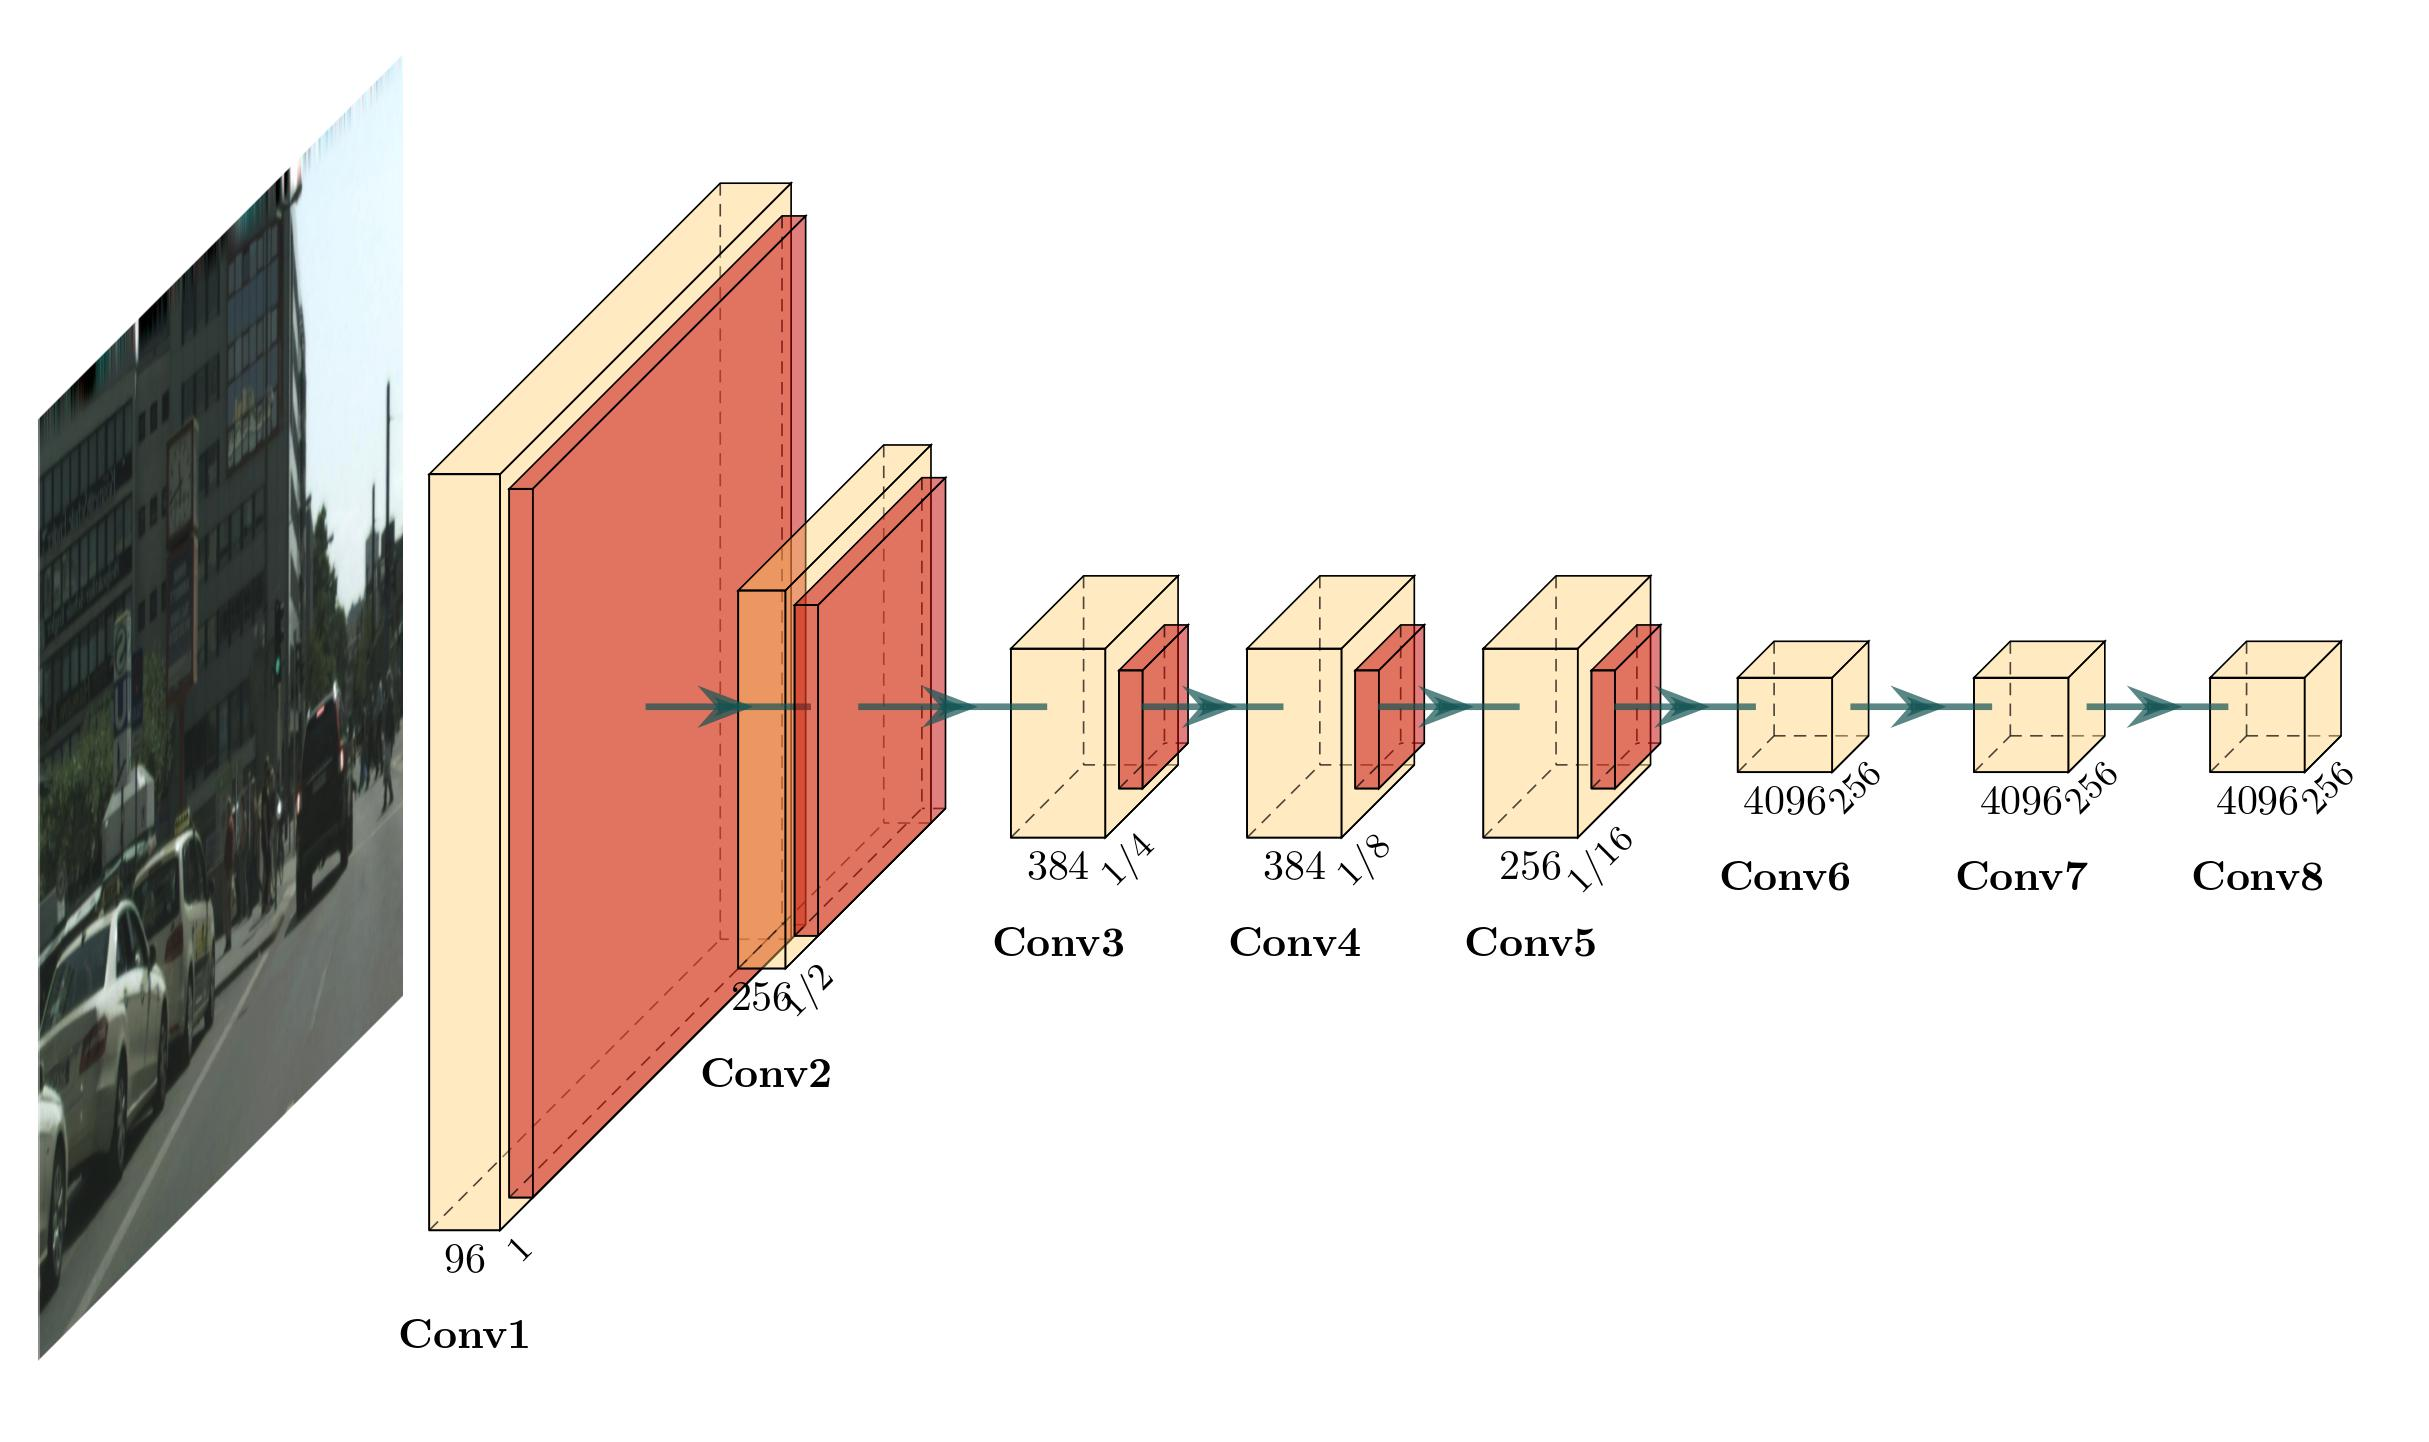
\includegraphics[width=1\textwidth]{figures/FCN.png}
%         \caption{FCN structure: FCN can accept input images of any size, and use the deconvolution layer to upsample the heat map of the last convolution layer to restore it to the same size as the input image, thus producing a prediction for every pixel.}\label{FCN}
%     \end{subfigure}
%     \caption{CNN structure compared with FCN structure}\label{FCN-CNN}
% \end{figure}


% The process of transmitting data from the bottom layer to the upper layer is called forward propagation. After the prediction result is obtained, it is compared with the ground truth, and the difference with the ground truth is obtained by calculating the loss. Then, by propagating the loss forward and updating the weight value of each layer of the network, the learning of the image is realized. This process is called backpropagation.

% % \begin{figure}[htb]
% %     \centering
% %     \includegraphics[width=1\textwidth]{figures/CNN.png}
% %     \caption{Typical CNN network structure: Usually, the CNN network will be connected to several fully connected layers after the convolutional layer, and the feature map generated by the convolutional layer will be mapped into a fixed-length feature vector. The classic CNN structure represented by AlexNet is suitable for image-level classification and regression tasks, because they all expect a numerical description (probability) of the entire input image at the end. For example, AlexNet's ImageNet model outputs a 1000-dimensional vector indicating that the input image belongs to Probability of each class (softmax normalization)}\label{CNN}
% %     % 图片的标题应该在下方
% % \end{figure}



% The FCN is not connected to the traditional fully connected layer after the convolutional layer, but a deconvolutional layer, which performs the function of upsampling and restores the obtained data to the size of the input image, to obtain a pixel-level semantic segmentation image of the original size. In the process of pooling, 1/2, 1/4, 1/8, 1/16, and 1/32 size relative to the original size image will get. 1/8, 1/16, and 1/32 images will be used for the upsampling operation. 

% Among them, 1/32 of the images mainly contain the most abstract semantic information of the original image, and thus the result obtained by direct upsampling is also the most blurred and smooth. For the same reason, upsampling results of 1/8 images are better than 1/16 images, and 1/16 images are better than 1/32 images. Because the results obtained by direct upsampling of pooling images are not ideal, the author proposes a series of upsampling networks that integrate images of various sizes, including FCN-8s, FCN-16s, FCN-32s.

% \begin{figure}[htb]
%     \centering
%     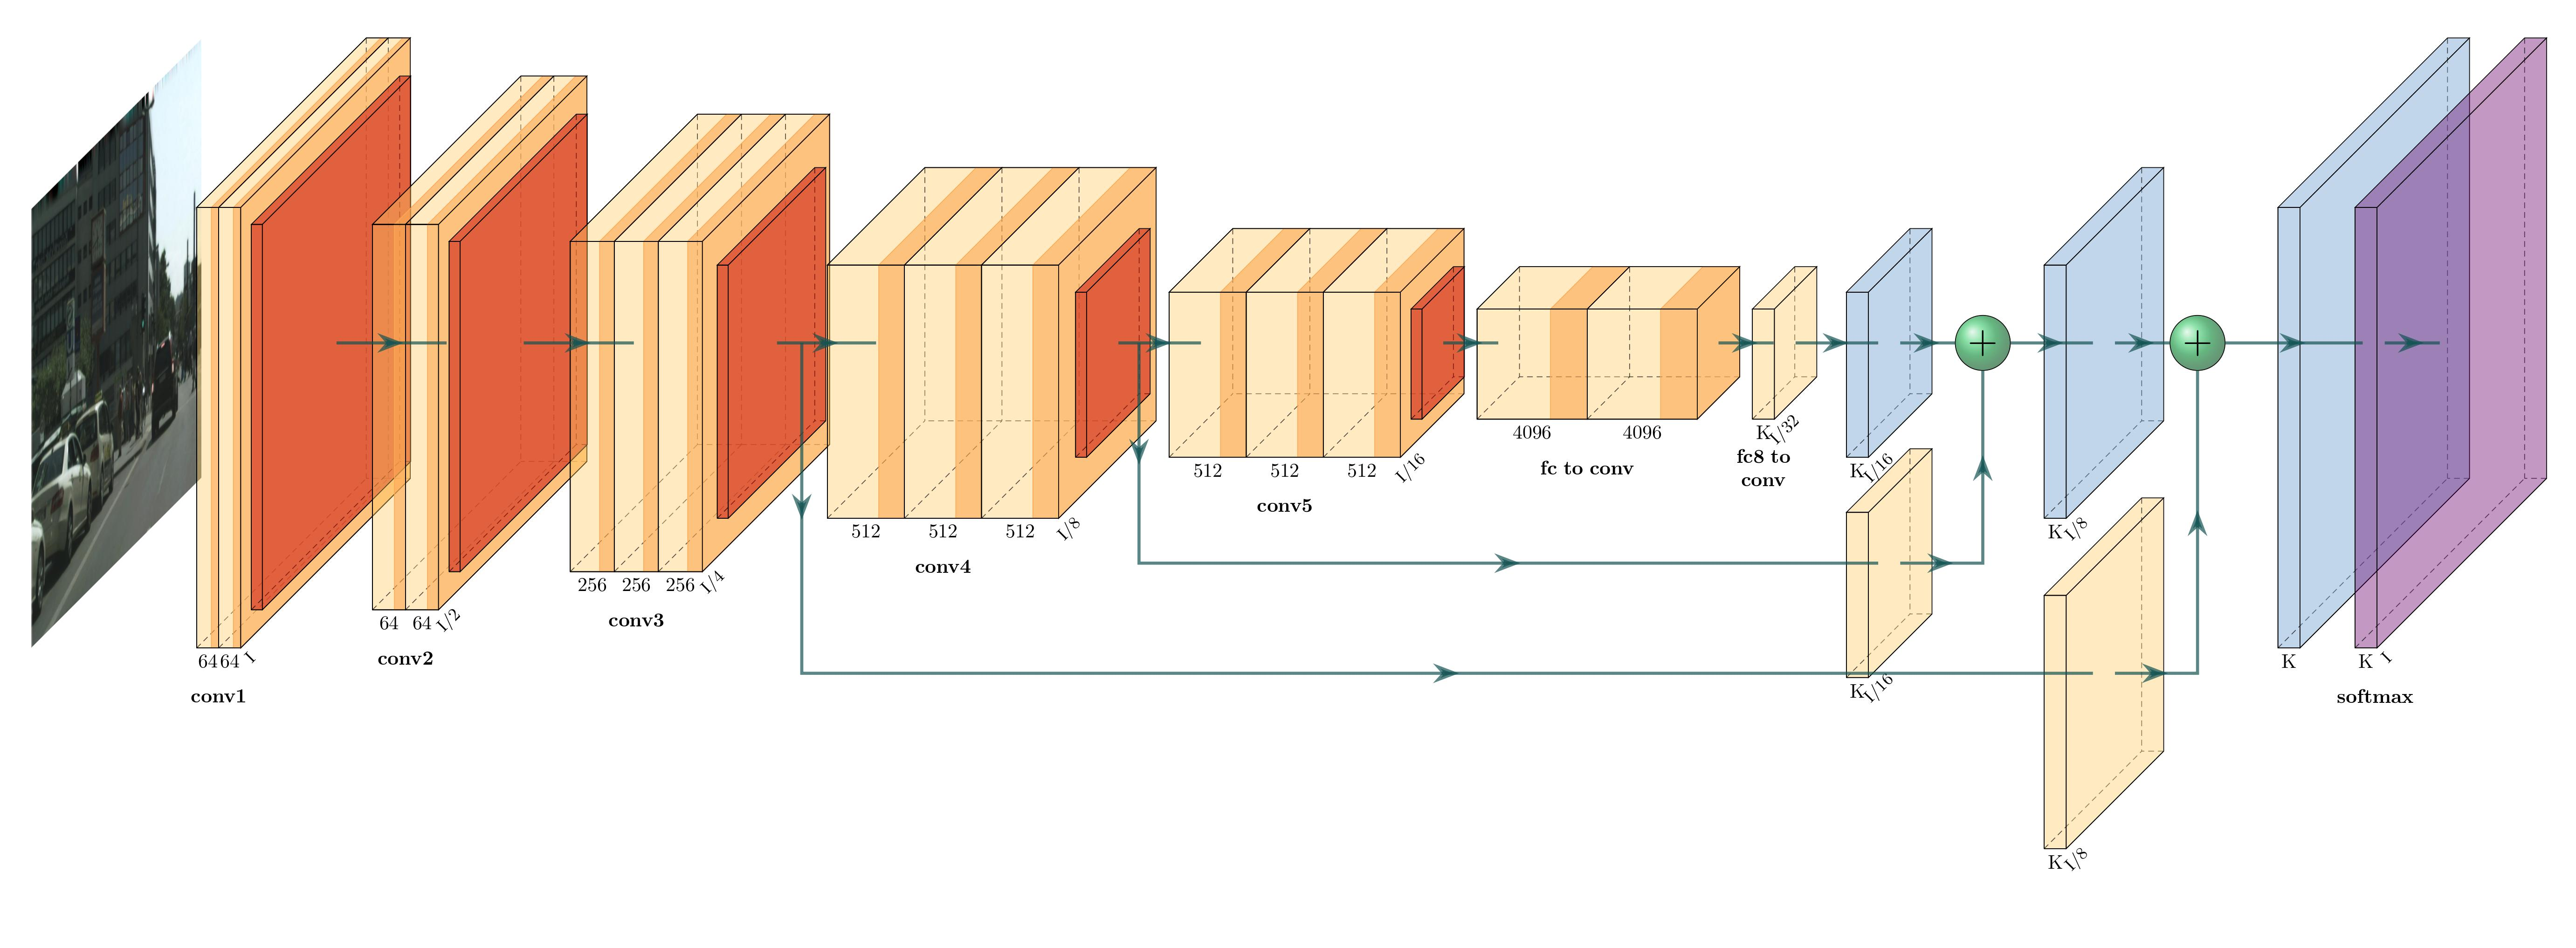
\includegraphics[width=1\textwidth]{figures/FCN8.jpg}
%     \caption{FCN-8s' Structure \cite{plotNeuralNet}}\label{FCN8}
% \end{figure}

% Among them, FCN-8s and FCN-16s use a skip-level structure to ensure the correctness of the results. By comparing the three-stage training results, FCN-8s, which utilize all levels of semantic information, have the most refined results.

% FCN innovatively uses a deconvolution layer to replace the fully connected layer and obtains pixel-level semantic segmentation results for input images of any size, and the results are better than state-of-the-art. However, the result of upsampling is not sensitive to the details of the picture, and the obtained result still has the problem of being too smooth and blurred. At the same time, the subsequently proposed ResNet50 and ResNet101 use the FCN network to improve the idea of ​​the fully connected layer and improve the effect of semantic segmentation through the residual network.

% However, compared with FPN and FaPN, FCN still has insufficient utilization of multi-level semantic information in the utilization of semantic information, and its network has many layers and a large number of parameters, so it is not suitable for porting to mobile terminals for real-time semantic segmentation.


\subsection{Feature Pyramid Networks}
Feature Pyramid Networks \cite{lin2017feature} is an article published in CVPR by Tsung-Yi Lin et al. in 2017. It integrates the semantic information of the bottom layer and the upper layer by adding a feature pyramid module to the Dense prediction problem and improves the accuracy of target detection, especially for the detection of small objects.

\begin{figure}[htbp]
    \centering
    \begin{subfigure}[t]{0.3\linewidth}
        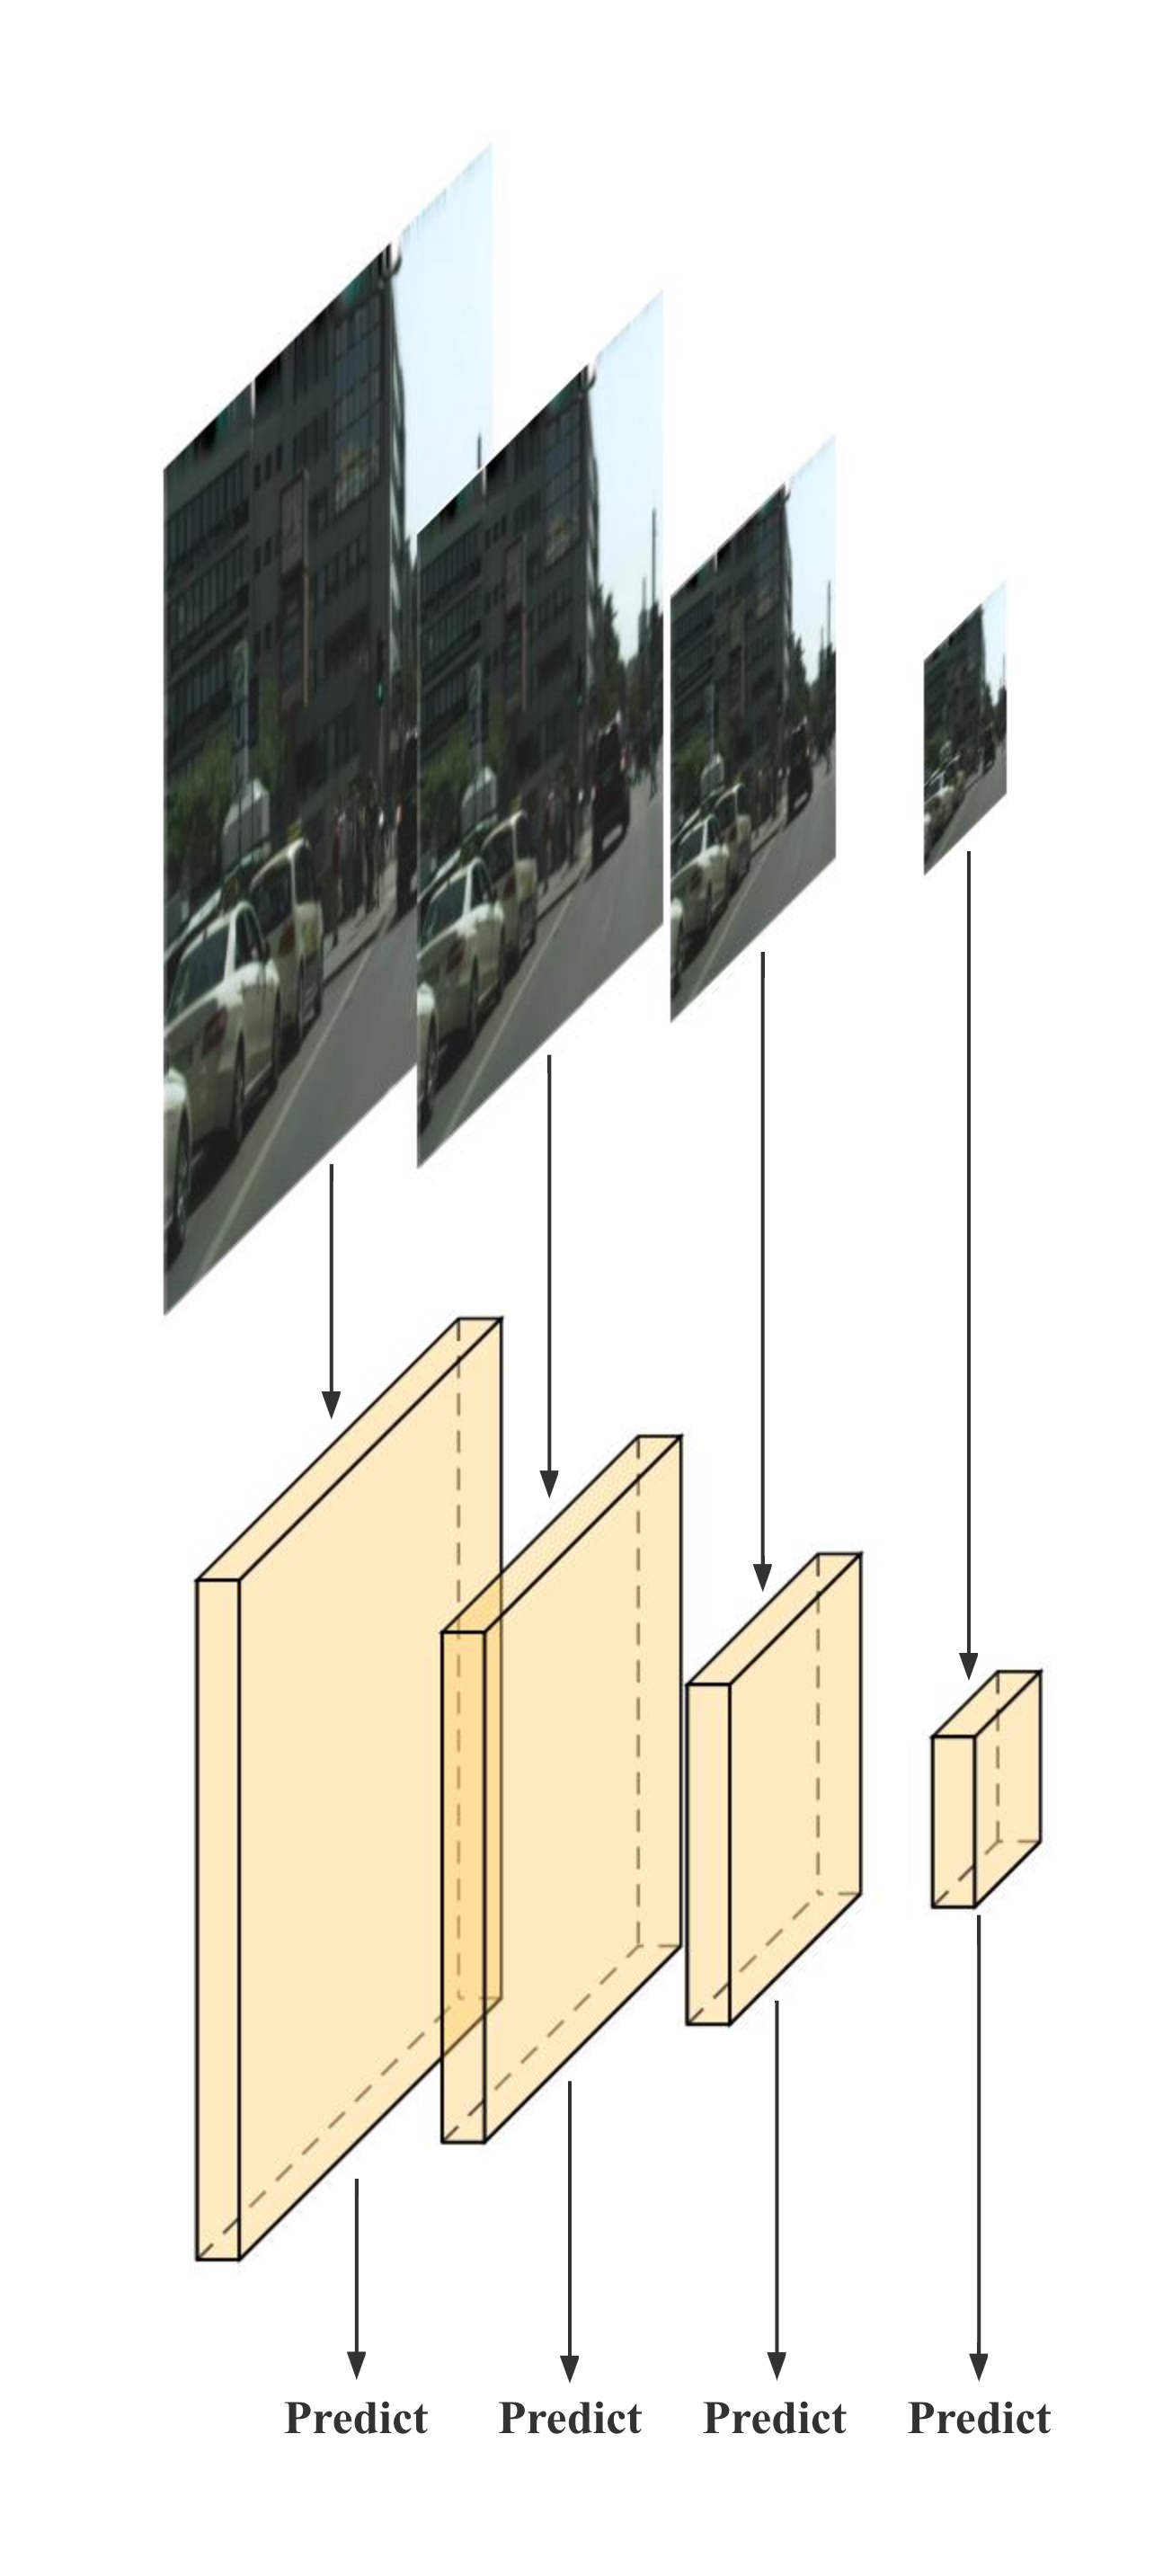
\includegraphics[width=1\textwidth]{figures/fcnarch1.png}
        \caption{Featurized Image Pyramid}\label{FCNarch1}
    \end{subfigure}
    \begin{subfigure}[t]{0.3\linewidth}
        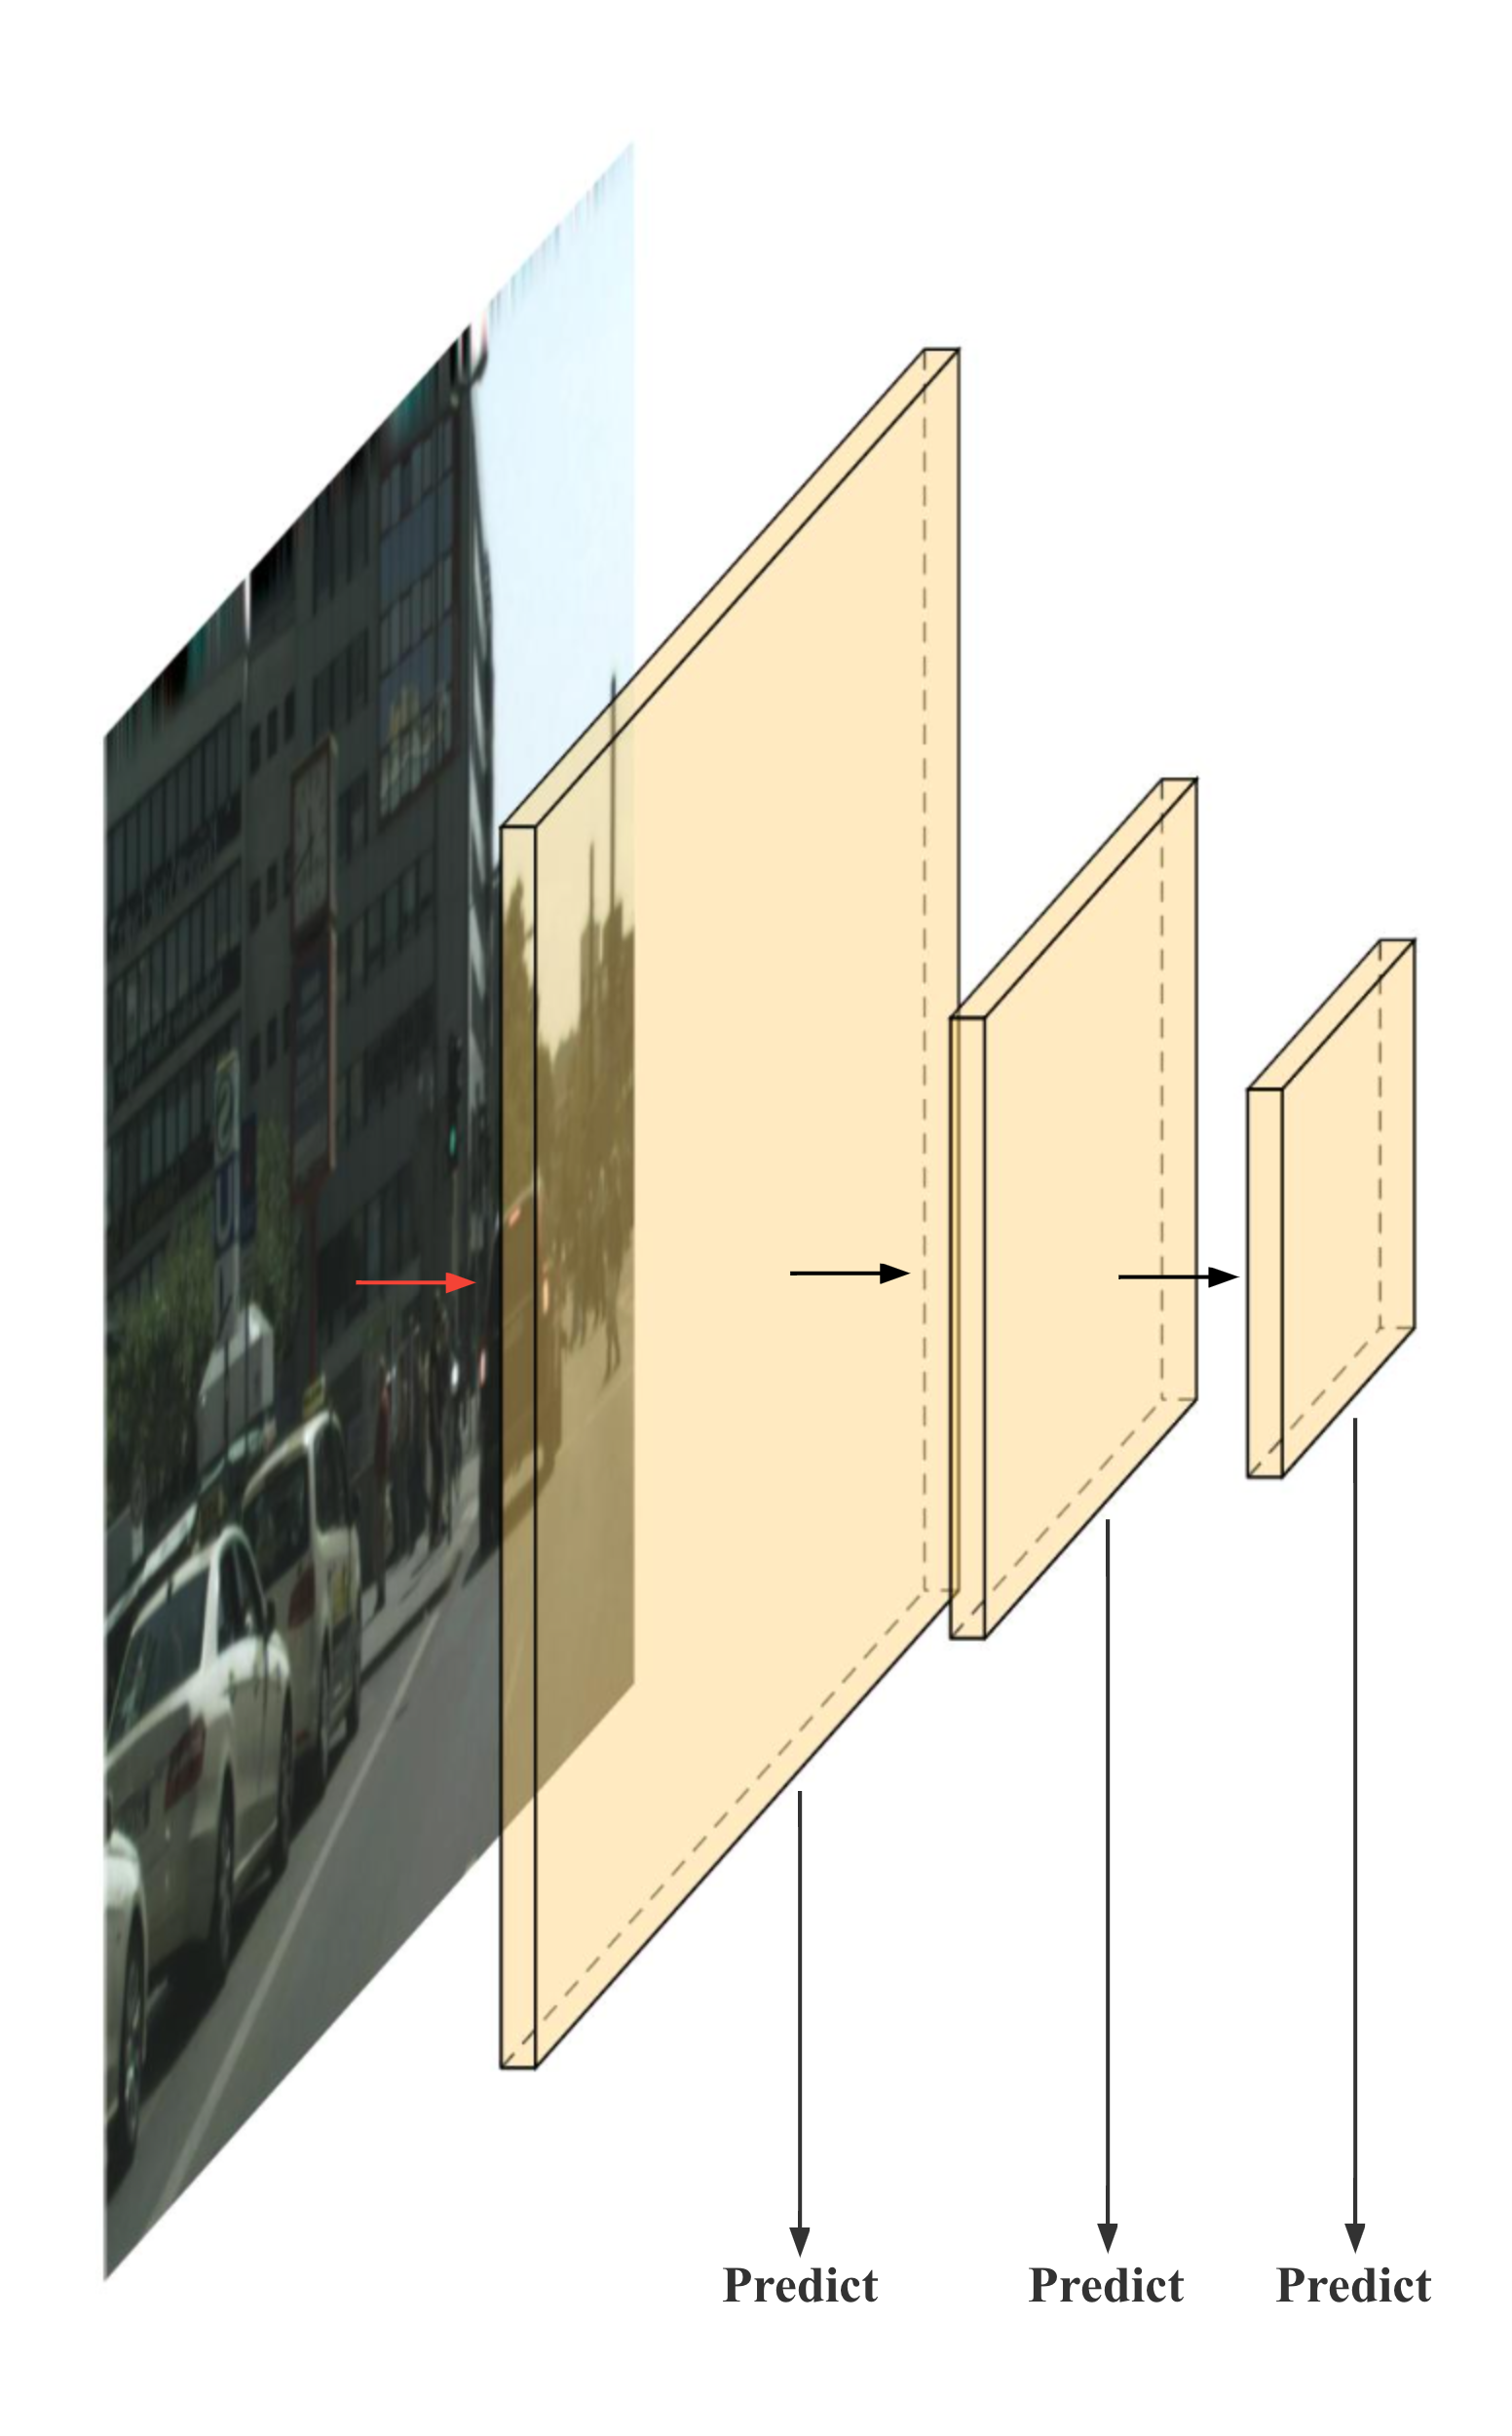
\includegraphics[width=1\textwidth]{figures/fcnarch2.png}
        \caption{Pyramid Feature Hierarchy}\label{FCNarch2}
    \end{subfigure}
    \begin{subfigure}[t]{0.3\linewidth}
        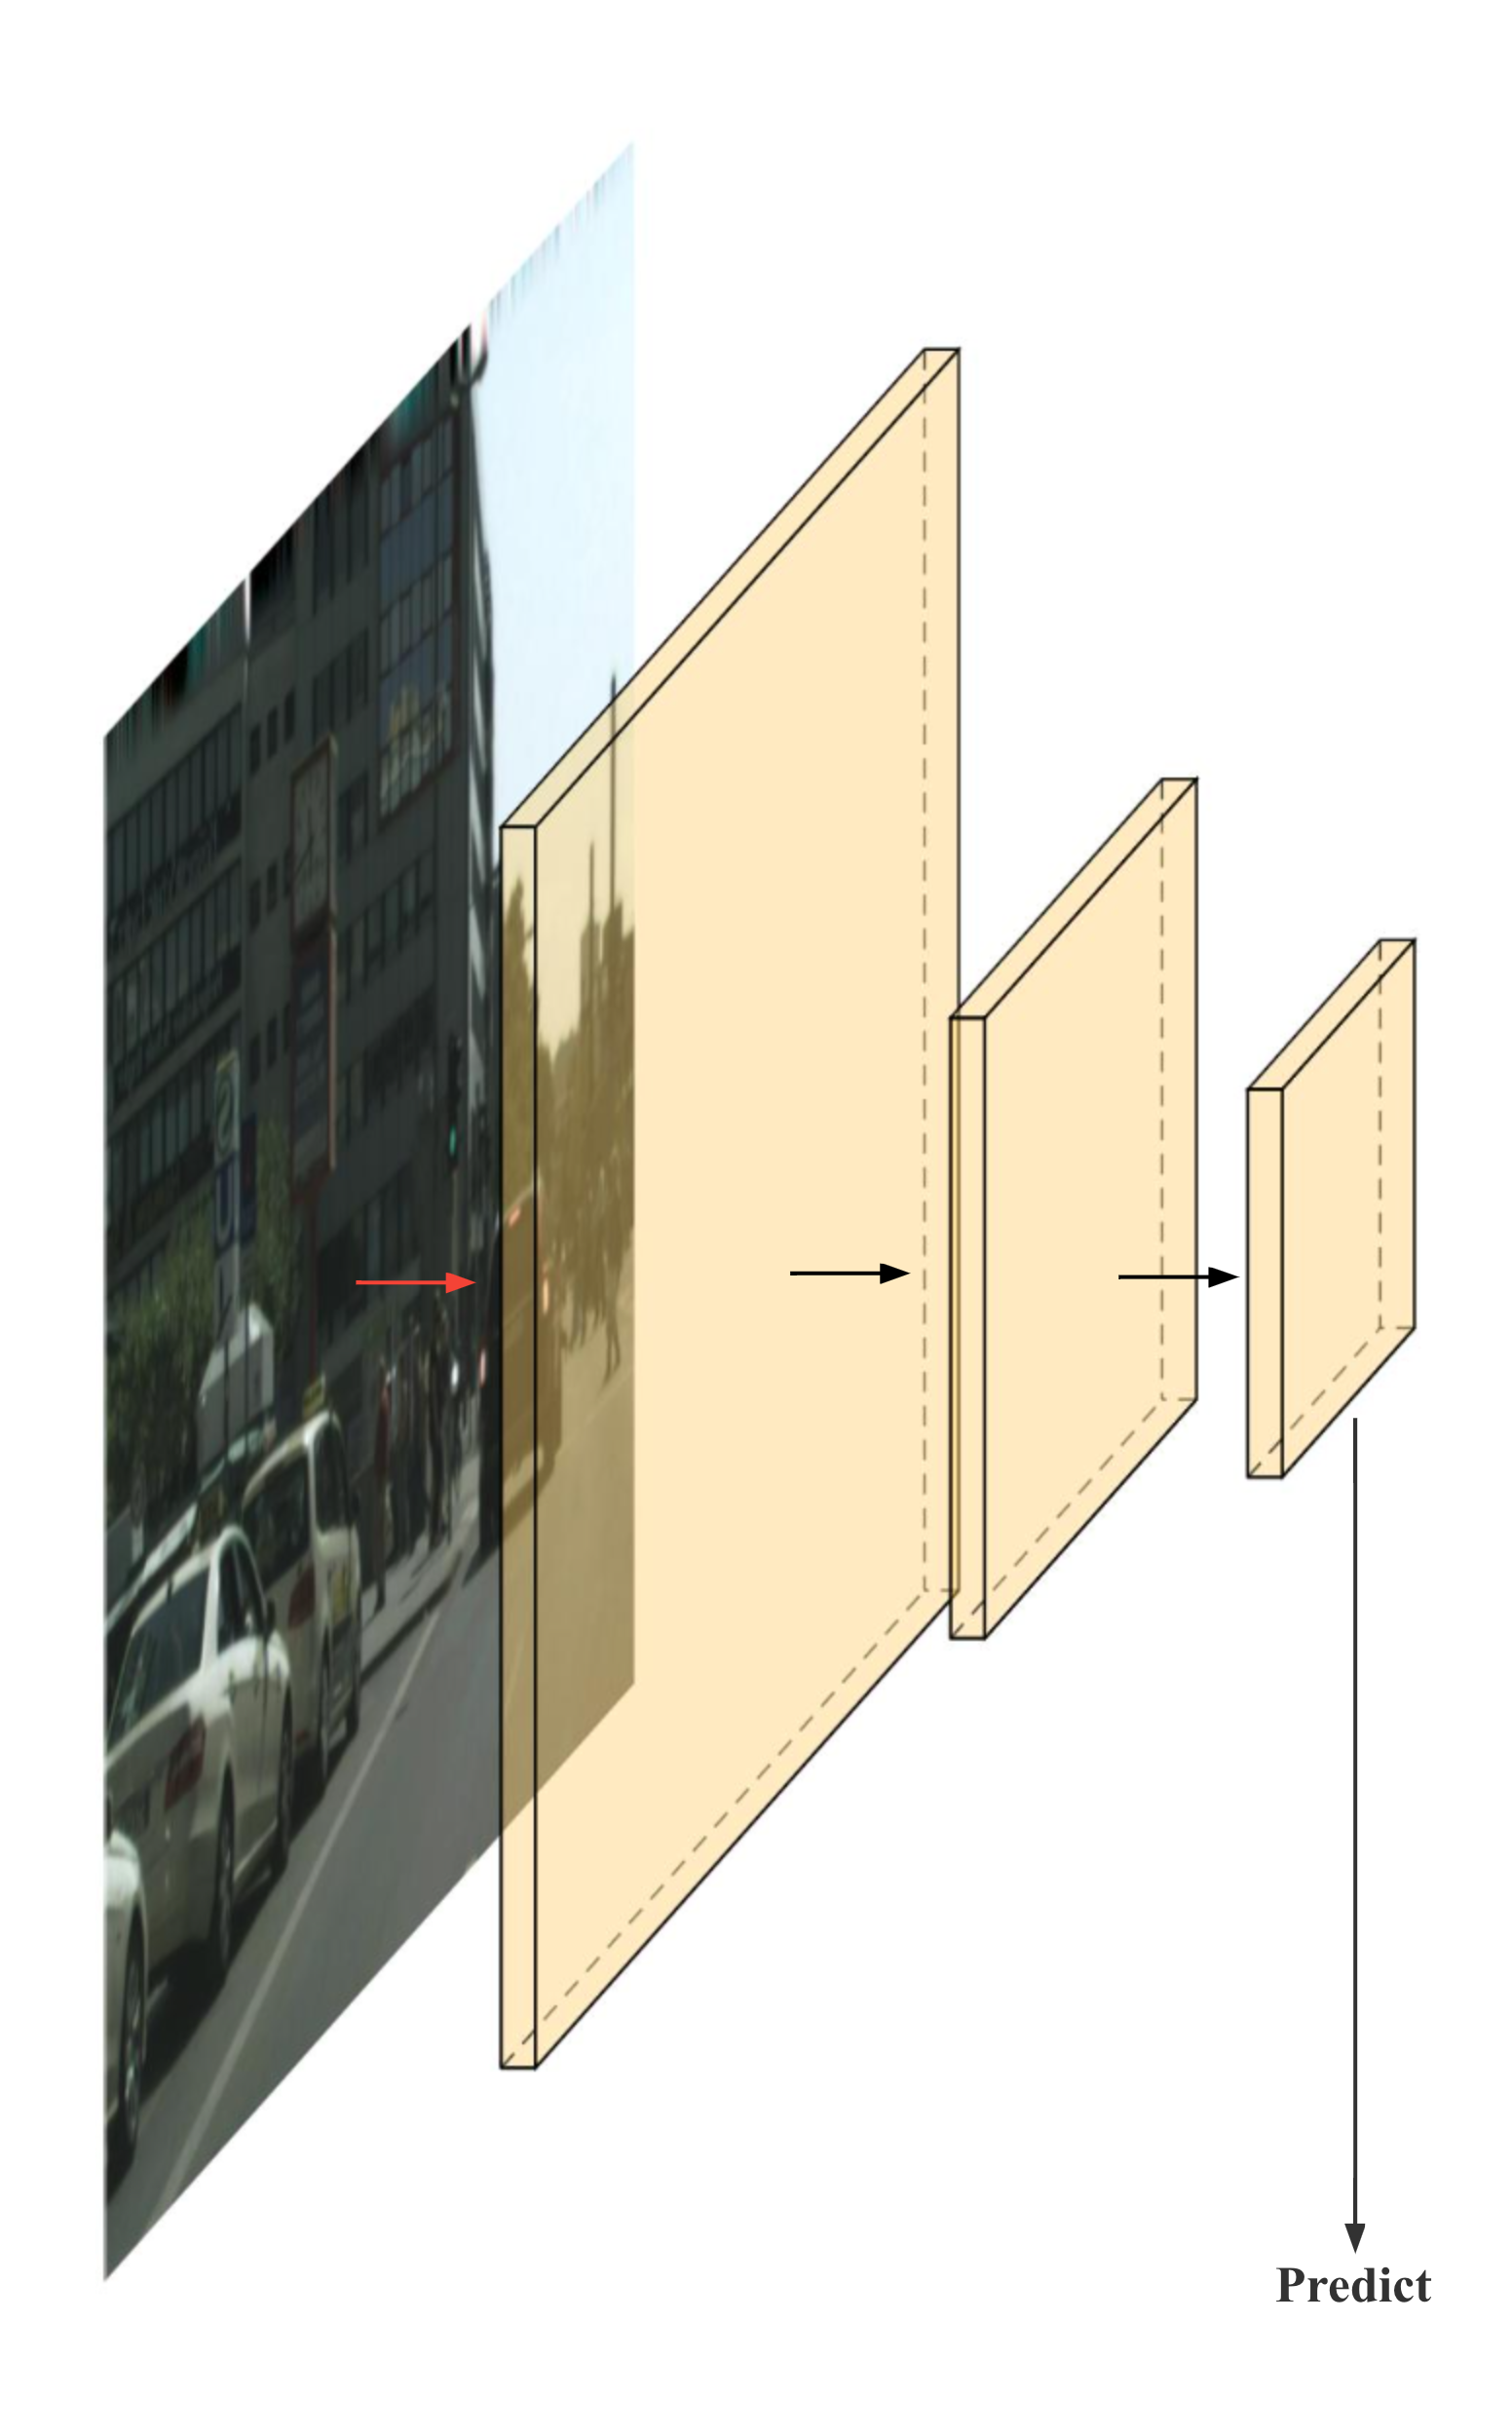
\includegraphics[width=1\textwidth]{figures/fcnarch3.png}
        \caption{Single Feature Map}\label{FCNarch3}
    \end{subfigure}
    \caption{Three typical  structures in target detection}\label{FCNarch}
\end{figure}


There are three typical structures in object detection: a) Featurized image pyramid, b) Pyramid feature hierarchy, and c) Single feature map. Among them, the Featurized image pyramid obtains the features of different scales through images of different resolutions and makes separate predictions for the features of each scale. The problem is that the time cost is too high. The pyramid feature hierarchy extracts different levels of semantic information from images through the network and predicts them separately. In this way, when high-level semantic information is used, the detection effect of small objects is not good. A single feature map only predicts the feature map of the highest layer of the network, but the resolution of the feature map of the highest layer is low, and the prediction of the position of the object is not accurate enough.

\begin{figure}[htbp]
    \centering
    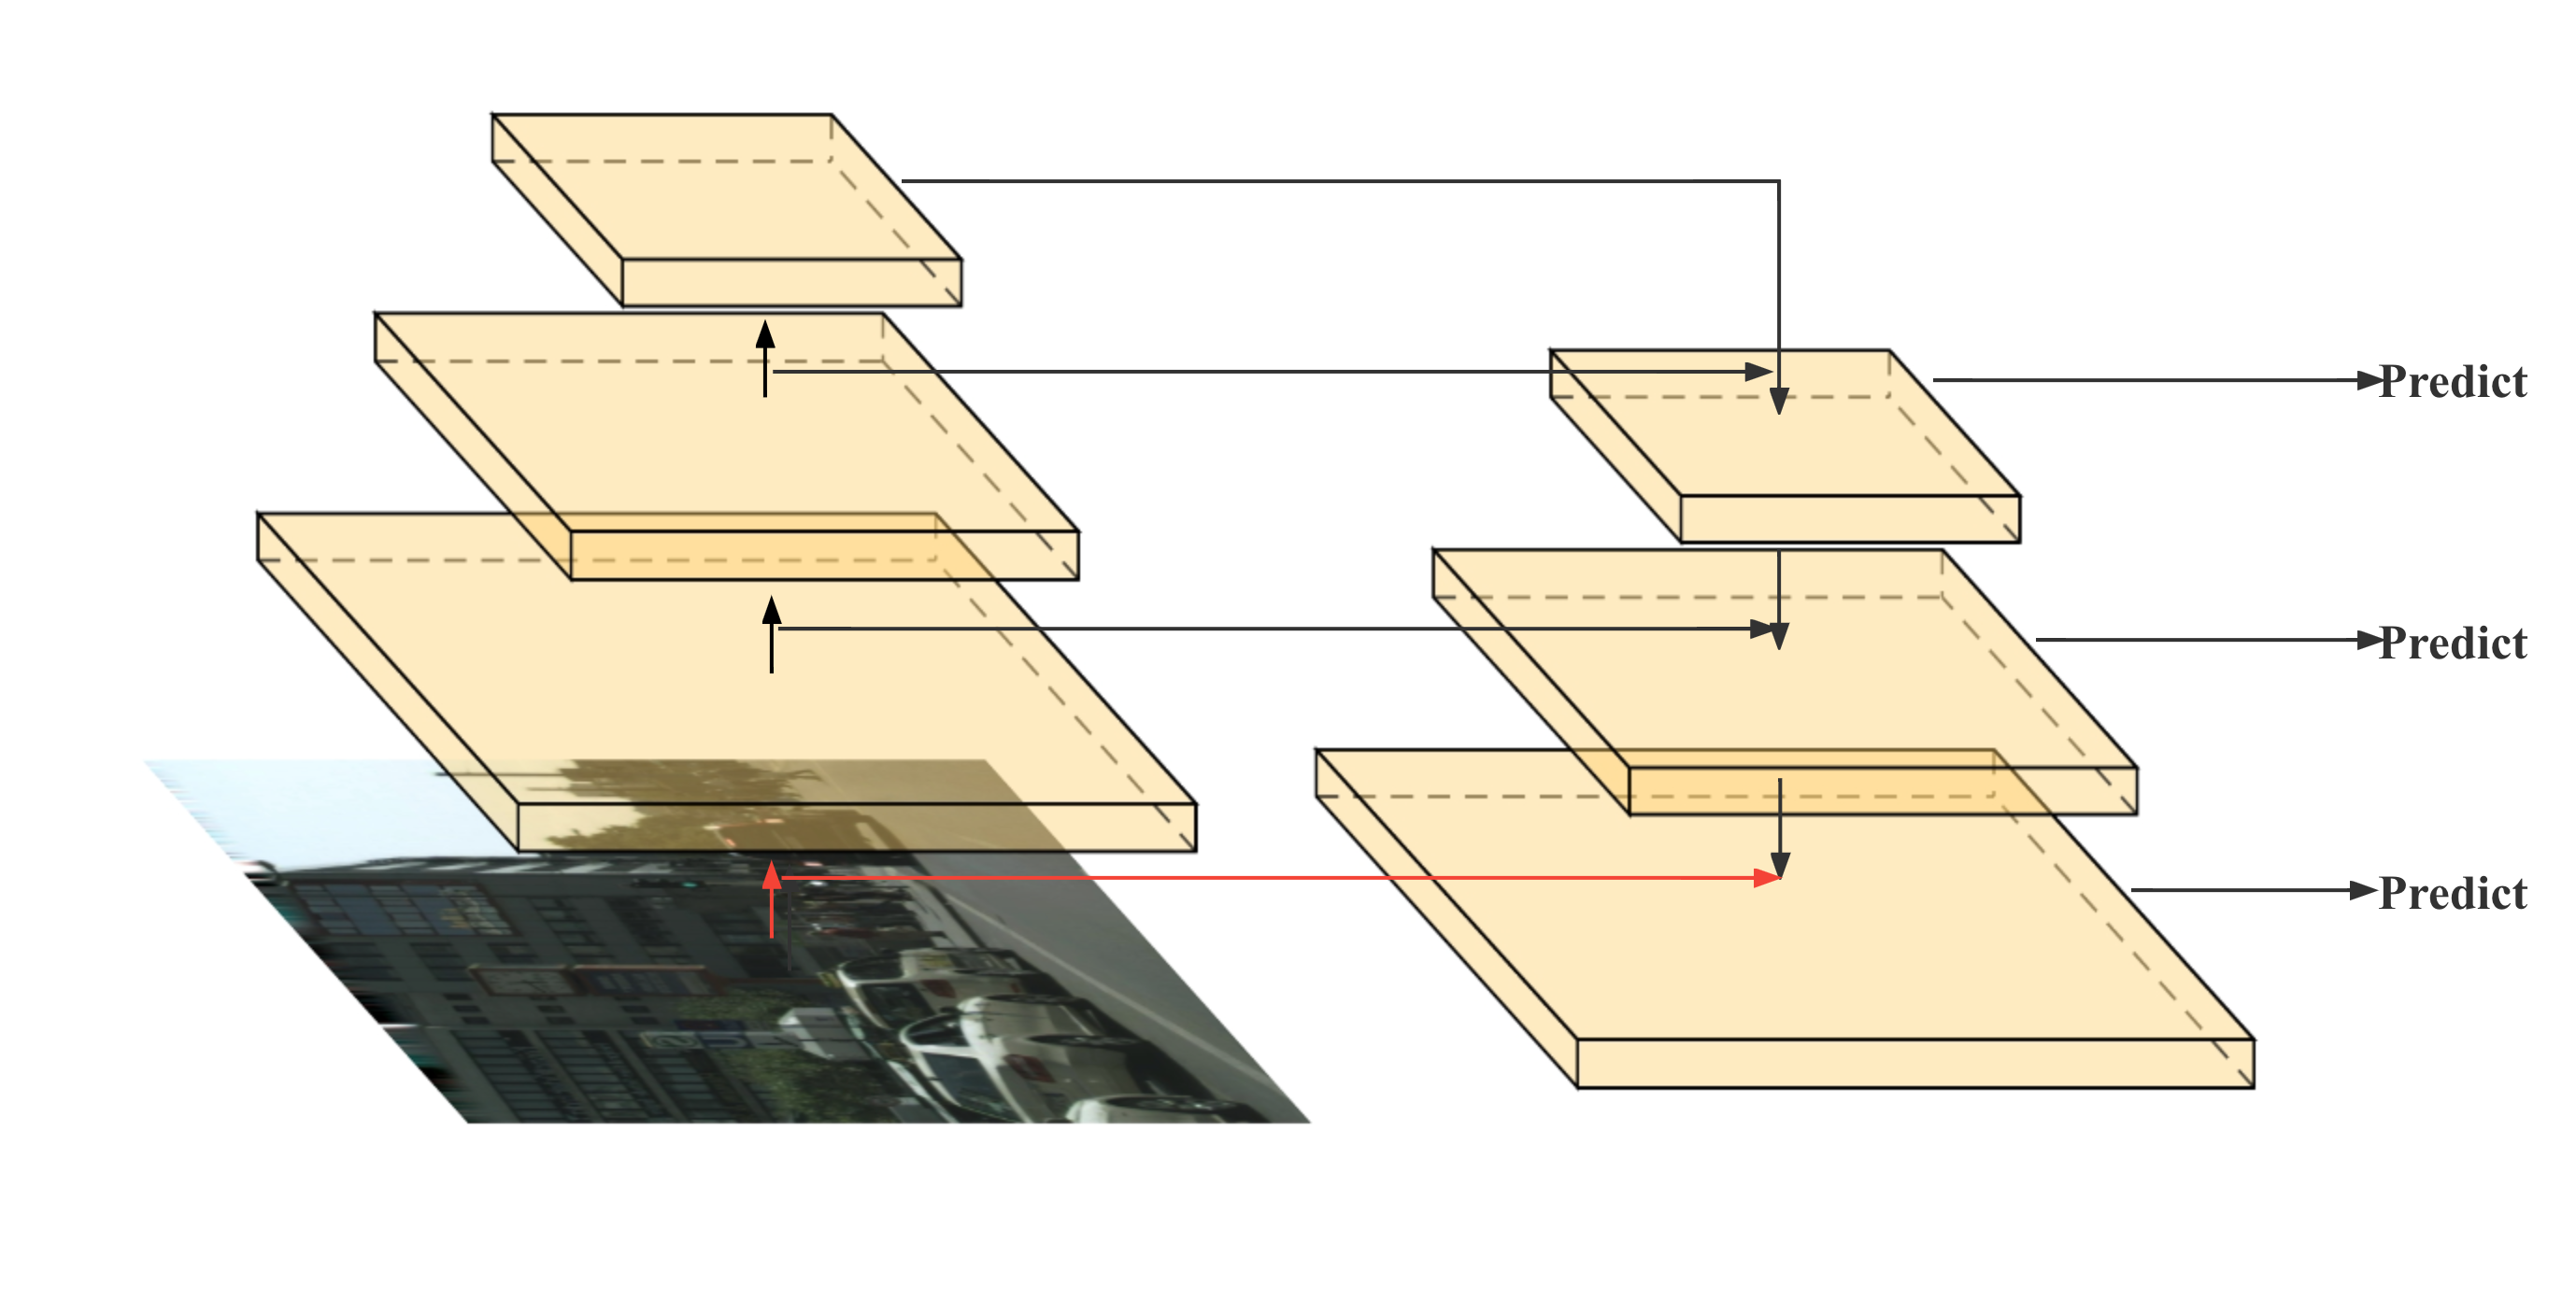
\includegraphics[width=1\textwidth]{figures/FPN_h.png}
    \caption{FPN's Structure \cite{plotNeuralNet}}\label{FPN}
\end{figure}

The FPN network uses the top-down pathway to combine the feature information of the bottom layer and the upper layer resolution. By upsampling, the more abstract high-level feature map and laterally connecting it with the lower-level feature map, the feature information of the high-level layer is strengthened. In this way, the feature information of the upper layer and the position information of the bottom layer is used at the same time, thereby improving the accuracy of dense prediction, especially for the prediction of small objects.


\subsection{Feature-aligned Pyramid Networks}

Based on FPN, Shihua Huang further proposed Feature-aligned Pyramid Networks \cite{huang2021fapn}. FPN and most of the existing networks do not consider the problem of feature alignment, which leads to the upsampling of high-level semantics, and the upsampled local features are directly filled with pixels by interpolation methods. The interpolated pixel padding can lead to misalignment of the upper and lower layer features of small objects and object boundaries, which in turn leads to misclassification in prediction.

For the above problems, the author proposes FAM (Feature Alignment Module) and FSM (Feature Selection Module) to help the model obtain more accurate upper-level semantic location information.

%两个模块解释(伪代码放在实现部分):

%因为在上卷积层向下卷积层进行上采样的过程中存在特征无法对齐的问题,所以在上采样的过程中,作者通过添加的FAM模块对这些特征样本进行了对齐。具体过程如下
Because of the problem that the features cannot be aligned in the process of upsampling the upper convolutional layer and the down convolutional layer, the author aligns these feature samples through the added FAM module during the upsampling process. The specific process is as follows:

For a given upsampled feature map $P_i$, the spatial misalignment between it and the bottom-up feature map $C_i$ is predictable.


Unaligned upsampled layers' features and bottom-up feature maps' features may lead to the wrong prediction of upsampled layers' features in the process of recursive upsampling, which in turn leads to the wrong prediction of small objects and object edges, so the alignment of features in upsampled layers' $P_i$ and bottom-up feature maps' features $C_i$ is very necessary. The spatial location information, the offset $\Delta_i$ is provided by both the feature's location in $C_i$ and $P_i$. With the information provided, the aligned feature could be calculated according to the offset $\Delta_i$ and unaligned feature $P^u_i$ in upsampled layer $P_i$. The mathematical formulation is present as in Equation (\ref{con:FAM}) \cite{huang2021fapn}

\begin{equation}
    \begin{aligned}
        \Delta_i = f_a([\hat{\textbf{C}}_{i-1}, \textbf{P}^u_i]),\\
    \hat{\textbf{P}}^u_i = f_m(\textbf{P}^u_i, \Delta_i),
    \label{con:FAM}
    \end{aligned}
\end{equation}

where $\Delta_i$ denotes the offset distance from the unaligned feature $C_i$ to the $P^u_i$, in which the $\hat{C}_{i-1}$ denotes the reference of $C_i$. $f_b(·)$ denotes the calculation procedure of the aligned feature $\hat{P}^u_i$. The algorithm is implemented by the deformable convolutions \cite{dai2017deformable}.


In the typical FPN, the bottom-up feature maps are added with the upsampled feature maps after a 1 * 1 convolutional layer. Thus, it's necessary to selectively use the useful feature. The mathematical formulation is present as in Equation(\ref{con:FSM}) \cite{huang2021fapn}

\begin{equation}
    \begin{aligned}
    \textbf{u} = f_m(\textbf{z}),\\
    \hat{\textbf{C}}_i = f_s(\textbf{C}_i+\textbf{u}*\textbf{C}_i),
    \label{con:FSM}
    \end{aligned}
\end{equation}

where the \textbf{u} indicates the importance vector, for each feature map there's an importance value to add all up. The importance value is extracted according to Equation(\ref{con:AVEPOOL}) \cite{huang2021fapn}

\begin{equation}
    \begin{aligned}
    \textbf{z}= [z_1, z_2, ..., z_D],\\
    \textbf{z}_d = \frac{1}{H_i * W_i}\sum_{h = 1}^{H_i}\sum_{w = 1}^{W_i}c_d(h,w),
    \label{con:AVEPOOL}
    \end{aligned}
\end{equation}

%这个平均池化的操作保证了对于feature map的重要特征的提取和提取后的一致性。使重要的特征得到了增强,不重要的特征被减弱。
This average pooling operation ensures the extraction and consistency of the important features of the feature map after extraction. The important features are enhanced, and the unimportant features are weakened.

% \subsection{Paddle Lite}
% Paddle Lite \cite{paddlelite} is an end-to-end reasoning engine launched by Paddle Mobile based on the new upgrade of Paddle Mobile. It is more complete in the support of multi-hardware, multi-platform and hardware hybrid scheduling, and provides efficient and lightweight AI applications for end-side scenarios including mobile phones. Reasoning ability, effectively solve problems such as mobile phone computing power and memory limitations, and are committed to promoting the wider implementation of AI applications.

\clearpage